%BEGIN_FOLD
%----------------------------------------------------------------------------------------
%   PACKAGES AND OTHER DOCUMENT CONFIGURATIONS
%----------------------------------------------------------------------------------------

\documentclass[12pt, a4paper, twocolumn, fullpage]{article}
\usepackage{algorithm}
\usepackage{float}
\usepackage{makecell}
\usepackage{color}
\usepackage{graphicx}
\usepackage{amssymb}
\usepackage{amsthm}
\usepackage{lipsum}
\usepackage{algorithmic}
\usepackage{subcaption}
%\usepackage[round]{natbib} TODO in future
\usepackage{titlesec}
\titleformat*{\section}{\Large\bfseries}
\titleformat*{\subsection}{\large\bfseries}

\usepackage{amsmath,amsfonts,amssymb,amsthm,epsfig,epstopdf,titling,url,array}


\theoremstyle{plain}
\newtheorem{thm}{Theorem}[section]
\newtheorem{lem}[thm]{Lemma}
\newtheorem{prop}[thm]{Proposition}
\newtheorem*{cor}{Corollary}

\theoremstyle{definition}
\newtheorem{defn}{Definition}[section]
\newtheorem{conj}{Conjecture}[section]
\newtheorem{exmp}{Example}[section]

\theoremstyle{remark}
\newtheorem*{rem}{Remark}
\newtheorem*{note}{Note}

%---------
%   ARTICLE INFORMATION
%----------------
\title{PRO3DCNN: convolutional neural network for mapping protein structure into folds}
\author{Yechan Hong, Jan Segert, and Jianlin Cheng
\and University of Missouri, Columbia}
\date{\today}
%END_FOLD
\begin{document}
\tableofcontents
\maketitle

% ====================================
\section*{Abstract}
% ====================================

\textbf{Motivation:} SCOPe 2.07 is a database of 276,231 protein domains that have been partitioned into varying folds according to their shape and function. Since a protein's fold reveals valuable information about it's shape and function, it is important to find a mapping between protein's and it's fold. There are existing techniques to map a protein's sequence into a fold \cite{deepsf} but none to map a protein's shape into a fold. We focus on the topological features of a protein to map it into a fold. We introduce several new techniques that accomplish this.
\\
\textbf{Results:} We develop a 2D-convolutional neural network to classify any protein structure into one of 1232 folds. 
We extract two classes of input features for each protein's carbon alpha backbone: distance matrix and the persistent homology barcodes. Due to restrictions in our computing resources, we make sample every other point in the carbon alpha chain. We find that it does not lead to significant loss in accuracy.
Using the distance matrix, we achieve an accuracy of 86\% on the entire dataset.

We extract significant topological simplices of the protein by using persistent homology. We format the persistent homology data into various input features: persistence images \cite{persistenceImages}, simplex distance map, and simplex grouping.  With persistence images of 100x100 resolution, we achieve an accuracy of 62\% on SCOP 1.55. With simplex distance maps of 100x100 resolution, we achieve an accuracy of 70\%.
    
%   We also combine the different classes of input features to achieve an accuracy of :TODO\%. An analysis on the network is performed to qualitatively describe the features the network is using to accurately classify the proteins.

% ====================================
\section{Introduction}
% ====================================
\begin{figure*}[t]
	\centering
    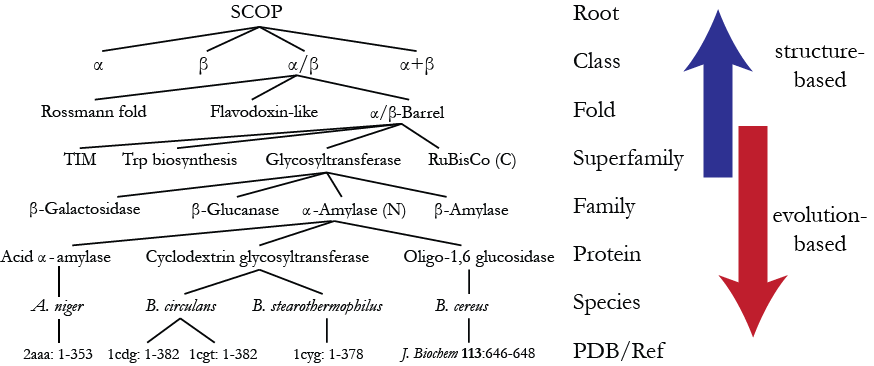
\includegraphics[width=.8\linewidth]{img/SCOP/scop_hierarchy.png}
    \caption{A partial view of the SCOP hierarchy.}
    \label{}
\end{figure*}

Structural Classification of Proteins (SCOP) is a database of protein structural relationships. The proteins are placed in an hierarchy in relative to their to structural and evolutionary relations \cite{scope}. 
SCOP was initially manually curated ordering of proteins \cite{scope}. However, as many numerous proteins continue to be discovered at a rapid pace, a need for an automatic method of classification became necessary.

Sequence based classification using deep convolutional neural networks like DeepSF show that it is possible to predict protein fold with an acurracy up to 75.3\% \cite{deepsf}. Structural Classification of Proteins - extended (SCOPe), extends the original SCOP database by using these types of rigorously validated automated methods to classify newly discovered proteins \cite{scope}. 

Similar to taxonomy, SCOP was created as a hierarchy with a basis in evolutionary relationships. Species, protein, family, and superfamily, the lower levels of the SCOP hierarchy represent the evolution-based relationships between the proteins. SCOP characterizes each of these levels with the following description \cite{scope}.

\begin{itemize}
   \item \textbf{Species} representing a distinct protein sequence and its naturally occurring or artificially created variants.
   \item \textbf{Protein} grouping together similar sequences of essentially the same functions that either originate from different biological species or represent different isoforms within the same species 
   \item \textbf{Family} containing proteins with similar sequences but typically distinct functions
   \item \textbf{Superfamily} bridging together protein families with common functional and structural features inferred to be from a common evolutionary ancestor.
\end{itemize}

Fold and class, the higher levels in our hierarchy as classified based on the similarity of structure and not necessarily evolutionary similarities \cite{scope}. 

\begin{itemize}
   \item \textbf{Folds} grouping structurally similar superfamilies.
   \item \textbf{Classes} based mainly on secondary structure content and organization.
\end{itemize}

The highest level of the hierarchy, class, consists of 7 categories. Alpha proteins (a), beta proteins (b), alpha/beta proteins (c), alpha+beta proteins (d), multi-domain proteins (e), membrane and cell surface proteins and peptides (f), and small proteins (g). The original SCOP publication clarifies the members of class a-e \cite{SCOP}. Class (f) and (g)'s name are descriptive of their members.

\begin{itemize}
\item \textbf{Alpha proteins} For proteins whose structure is essentially formed by a-helices.
\item \textbf{Beta proteins} For those whose structure is essentially formed by b-sheets.
\item \textbf{Alpha/Beta proteins} For proteins with
a-helices and b-strands that are largely interspersed.
\item \textbf{Alpha+Beta proteins} For those in which
a-helices and b-strands are largely segregated.
\item \textbf{Multi-domain} For those with domains of different
fold and for which no homologues are known at
present.
\end{itemize}

Many works have been done on using the protein sequences and their evolutionary relationships with each other to predict the protein hierarchy. This is primarily due to the lack of structural information for newly discovered proteins. 

In this paper, we shift the focus from a protein's sequence to the topological structure to predict the protein's fold and class. We expect the shift in focus to be quite successful in classifying the protein class and fold since these levels have been curated based on the similarity of structures between the proteins.

Since each fold belongs to only one class, predicting the protein fold also predicts the protein's class. Thus, we narrow the focus of our problem to predicting a protein's fold.

We introduce two methods for classifying protein fold. First, we use a distance matrix as an input feature to a convolutional neural network. Second, we use persistent homology to extract topological features of our data and plot these features as an input feature to a convolutional neural network.
\\

\noindent
\textbf{Distance Matrix}\\
Each protein has a backbone structure that is formed by  series of connecting points. The backbone structure of the protein is characteristic of the protein's general shape. A distance matrix of the protein's backbone is created, where the rth row and cth column of the matrix gives the distance between the rth point and the cth point of the protein backbone. Then this matrix is used as an input to our convolutional neural network.

There has been existing work (Fast SCOP Classification) on using the distance matrix to classify proteins from a very small subset of SCOP database \cite{fastSCOP} of 698 proteins. The distance matrix is computed for the protein and fed into a multi-class support vector machine (SVM) of the One-Versus-One (OVO) variant. This approach achieved and accuracy of 74.55\% on this small subset of SCOP. 

We take a look at few of the representative proteins from alpha proteins, beta proteins, alpha/beta proteins, and alpha+beta proteins. We juxtapose each protein's distance matrix to the protein's structure to see if there are significant differences between the classes. We see that the distance matrices do represent the alpha helices, the beta sheets, and also the relationship between these features.

\begin{figure*}
	\centering
    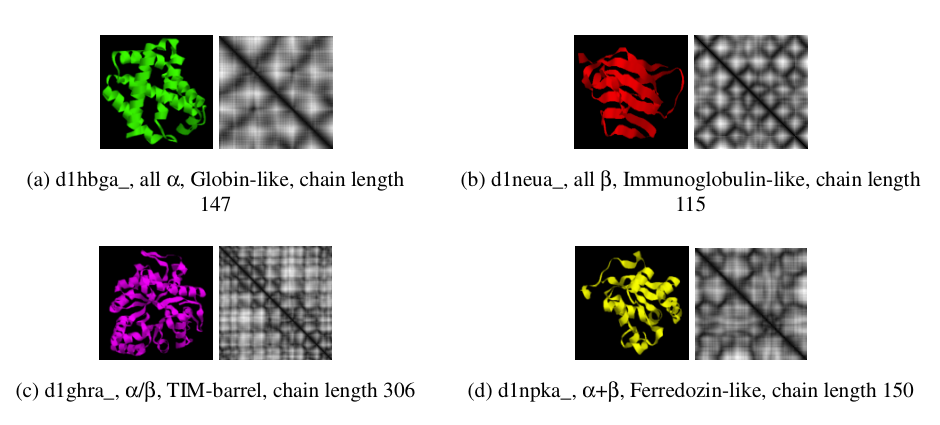
\includegraphics[width=\linewidth]{img/SCOP/scopDistCompare.png}
    \caption{A comparison of the distance matrix from the proteins of different classes. We see that the distance matrix is able to pick up on characteristic alpha helix and beta sheets of each protein, making it likely that this feature will perform well.}
    \label{}
\end{figure*}

\begin{figure}
	\centering
    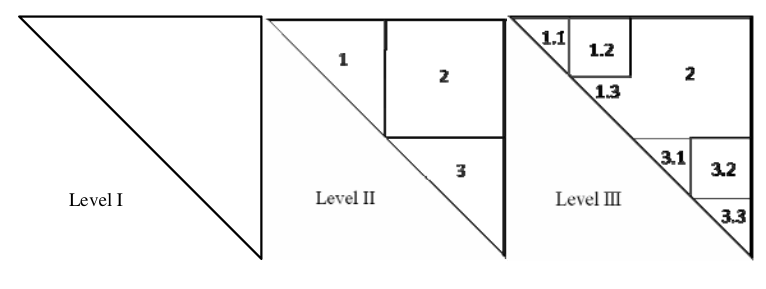
\includegraphics[width=.9\linewidth]{img/fastSCOP/ROIdecomp.png}
    \caption{Fast SCOP Classification decomposing the upper triangle of a distance matrix into regions of interest (ROI) to extract important features such as alpha helices and beta sheets.}
    \label{}
\end{figure}


Fast SCOP Classification extracts regions of interest (ROI) from the distance matrix by decomposing the upper triangle of the distance matrix into ROI. These regions attempt to capture the regions of the distance matrix where there are alpha helices and beta sheets. The relationships between these regions of interest are abstracted into a feature set which is given to the SVM for fold classification.

In comparison to our method, we employ a convolutional neural network to have the model learn the ROIs on it's own. The CNN has much more advantages over the decomposition method because complex relationships between regions of interest can be modeled by the hidden layer. Also the regions of interests are dynamically formed as the model is trained. There aren't supervisions into constructing the high-level feature set of ROIs, allowing the model to learn complex behaviors that may elusive or be difficult to define clearly. However, a downside to the CNN is that it is very computationally intensive, requiring a long training time and a large set of data to learn effectively. \\

\begin{figure}
	\centering
    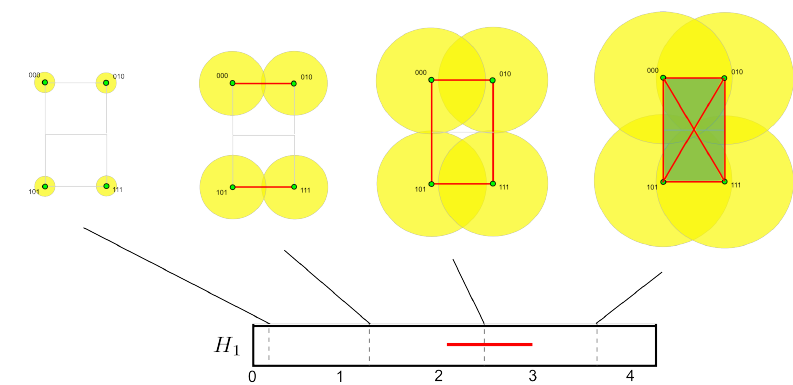
\includegraphics[width=\linewidth]{img/hom/persistentHomEx.png}
    \caption{Here is persistent homology characterizing the point cloud of four points. We see that a rectangular cycle is formed when the 4 boundary edges of the rectangles are formed at $\epsilon = 2.6$. We see that this rectangular cycle is dies at   $\epsilon = 3.4$}
    \label{fig:persistentHomEx}
\end{figure}

\noindent
\textbf{Persistent Homology}  \\
Persistent homology is a mathematical theory from algebraic topology that allows the characterization of a point cloud by the observing creations of cycles in the data and how long these cycles persist. We iterate over a real number variable, $\epsilon$, and connect the edges in our point cloud whose length is smaller than $\epsilon$. 

A cycle is formed when a closed loop is formed by the path of the edges. In the example with 4 points (Fig.\ref{fig:persistentHomEx}), a cycle is formed when the four edges of the rectangle's boundary is formed. The $\epsilon$ value at which the cycle is formed is called the $birth$ of this cycle. This cycle is destroyed when triangles a formed within our cycle to completely fill it in. The $\epsilon$ value associated with the cycle being filled in is called the $death$ of the cycle. We say that the cycle persists for a duration of $birth-death$. Each cycle forms an interval, $[birth, death]$. The collection of all intervals from the cycles in the data is called a barcode.

There has been existing attempts at using Persistent Homology to classify the highest level of SCOP hierarchy \cite{SCOPHom}. Cang applies persistent homology on a small set of 900 proteins selected from Alpha, Beta, and Alpha/Beta classes. Each class is represented by 300 proteins and 60 proteins were selected for testing. A SVM is used to classify the classes with with an average accuracy of 85\%. 

When we observe the barcode of the proteins from the different classes we do see some distinguishing patterns (Fig.\ref{fig:scopHom}). The proteins with alpha helices have a long curved edge towards the top of the barcode, while proteins with beta sheets have a thicker bar towards the bottom.

\begin{figure*}
	\centering
    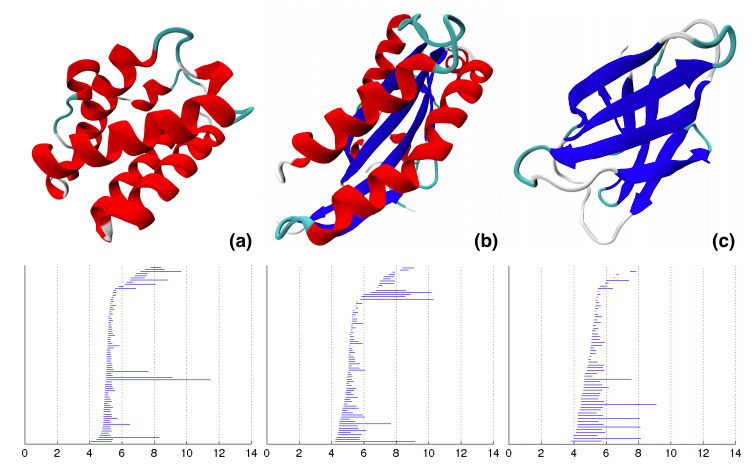
\includegraphics[width=.8\linewidth]{img/hom/scopHom.png}
    \caption{Persistent homology was used to calculate the barcodes on three proteins from Alpha protein (a), Alpha/Beta protein (b), Beta protein(c) classes. The proteins with alpha helices (red) have elongated structures at the top of the barcode while proteins with beta sheets (blue) are thick at the base.}
    \label{fig:scopHom}
\end{figure*}
 In comparison to our method, we classify proteins based on folds, a more specific level of the SCOP hierachy. Our task of classification is much more extensive than the classification task performed in Cang. We classify 276,231 proteins into 1232 labels compared to the 900 proteins into 3 labels. We also use a convolutional neural network as opposed to a SVM. 
 
In the examples we have discussed, we note that the distance matrices contains much more information than the barcodes. This difference is resolution may cause the matrices to perform better than the barcodes.

% ====================================
\section{Materials}
%====================================

%----------------------
\subsection{Datasets}
%----------------------

The SCOP and SCOPe database is a database of proteins organized into hierarchical classes based on their shape and function. There are 4 levels of the important hierarchy (top down): Class, Folds, Superfamily, Family. We will be primarily concerned with the Fold.

Two different versions of the dataset were used, SCOP 1.55 and SCOPe 2.07. SCOP 1.55 is a smaller dataset which is a subset of SCOPe 2.07, a larger and more recent dataset. SCOP 1.55  and SCOPe 2.07 were downloaded from the Berkeley repository as tar files and unpacked. For each of the datasets, index files are provided.

SCOPe 2.07 has about 8 times more entries than SCOP 1.55 as well twice the amount of protein folds that we need classify. The rapid growth of SCOP 1.55 to SCOPe 2.07 can be attributed to the use of automatic classification that was applied to assign hierarchy to newly discovered proteins. 

\begin{figure*}
	\centering
    \includegraphics[width=.9\textwidth]{img/SCOP/scopchanges.png}
    \caption{A graph of the development of our dataset from SCOP 1.55 to SCOPe 2.07}
    \label{SCOPchanges}
\end{figure*}

Because of computation restrictions early on our research, we could not apply our methods to the large SCOPe 2.07 dataset which had a unzipped size of about 40gb. The methods in our research initially started by applying fold classification on SCOP 1.55. Since SCOP 1.55 is a subset of SCOPe 2.07, there weren't any surprises in applying the methods from SCOP 1.55 to SCOPe 2.07. Later on our research, when we were developing new methods, we were able to follow this similar workflow of working in the smaller dataset and then applying our method on the larger dataset. This workflow allowed us to quickly prototype and optimize our methods before running it on the larger datset.


\subsubsection{Small Dataset SCOP 1.55}
\begin{table*}[h]
    \centering
    \begin{tabular}{| l | l | l | l |}
        \hline 
        Class & \makecell{Number \\ of folds} & \makecell{Number  \\ of superfamilies} & \makecell{Number \\ of families} \\ \hline
        a. Alpha proteins & 138 & 224 & 337 \\ \hline
        b. Beta proteins & 93 & 171 & 276 \\ \hline
        c. Alpha and Beta proteins (a/b) & 97 & 167 & 374 \\ \hline
        d. Alpha and beta proteins (a+b) & 184 & 263 & 391 \\ \hline
        e. Multi-domain proteins (alpha and beta) & 28 & 28 & 35 \\ \hline
        \makecell[l]{f. Membrane and cell surface \\ proteins and peptides} & 11 & 17 & 28 \\ \hline
        g: Small proteins & 54 & 77 & 116 \\ \hline
        \textbf{Total} & \textbf{605} & \textbf{947} & \textbf{1557}  \\ \hline
        \hline
    \end{tabular}
    \caption{ SCOP 1.55 statistics of 31474 entries}
    \label{}
\end{table*}

SCOP 1.55 is a dataset of 31,474 proteins that have been organized into 7 Classes, 605 Folds, 947 Superfamilies, and 1557 Families. The dataset was released and updated till 2001. This dataset is a subset of the SCOPe 2.07 dataset.


\begin{figure}
    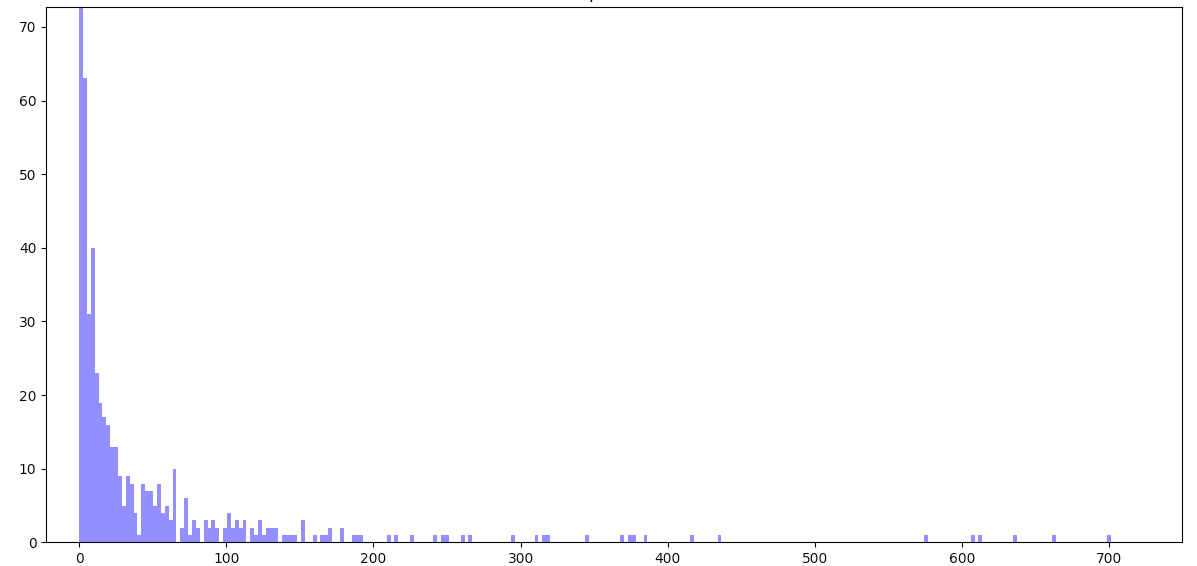
\includegraphics[width=\linewidth]{num_proteins_fold_155}
    \caption{Here is a histogram of the number of proteins per fold for SCOP 1.55. We see that most of the folds do not have too many proteins. This could be a potential issue during learning.}
    \label{num_proteins_fold_155}
\end{figure}

We inspect the distribution of the proteins across the different folds. We see that most of the folds do not have a lot of proteins. The median number of proteins per fold was 10 and the histogram (Fig.\ref{num_proteins_fold_155}) show that most of our proteins have less than 50 proteins per fold. This would likely impact our learning, since there are not too many examples for the protein to learn.


\begin{figure}
    \includegraphics[width=\linewidth]{chainlengths155}
    \caption{Here is a histogram of the protein lengths for SCOP 1.55. We see that 90\% of the proteins have length less than 500}
    \label{chainlengths155}
\end{figure}

We also inspect the length of the proteins in our database (Fig. \ref{chainlengths155}). We define the size of the protein to be the length of the protein (Background Information: Proteins Information). We see that most of the proteins have length less than 300. We do see a small amount of our proteins having lengths between 600 to 800. 

We split up 70\% of the dataset for training, 15\% for validation and 15\% for testing. We adjust the sampling of the validation and testing so that a wide range of folds are represented.

\subsubsection{Large Dataset SCOPe 2.07}

\begin{table*}[h]
    \centering
    \begin{tabular}{| l | l | l | l |}
        \hline 
        Class & \makecell{Number \\ of folds} & \makecell{Number  \\ of superfamilies} & \makecell{Number \\ of families} \\ \hline
        a. Alpha proteins & 289 & 516 & 1062 \\ \hline
        b. Beta proteins & 178 & 370 & 968 \\ \hline
        c. Alpha and Beta proteins (a/b) & 148 & 246 & 986 \\ \hline
        d. Alpha and beta proteins (a+b) & 388 & 565 & 1338 \\ \hline  \hline
        e. Multi-domain proteins (alpha and beta) & 71 & 71 & 118 \\ \hline
        \makecell[l]{f. Membrane and cell surface \\ proteins and peptides} & 60 & 119 & 173 \\ \hline
        g: Small proteins & 98 & 139 & 274 \\ \hline
        \textbf{Total} & \textbf{1232} & \textbf{2026} & \textbf{4919}  \\ \hline
        \hline
    \end{tabular}
    \caption{ SCOPe 2.07-stable statistics of 276231 entries. }
    \label{}
\end{table*}

SCOPe 2.07 is a database of 276,231 proteins that have been organized into 7 Classes, 1232 Folds, 2026 Superfamilies, and 4919 Families. The dataset was released and updated till 2017. This dataset contains and is about 9 times larger than the SCOP 1.55 dataset.

\begin{figure}
    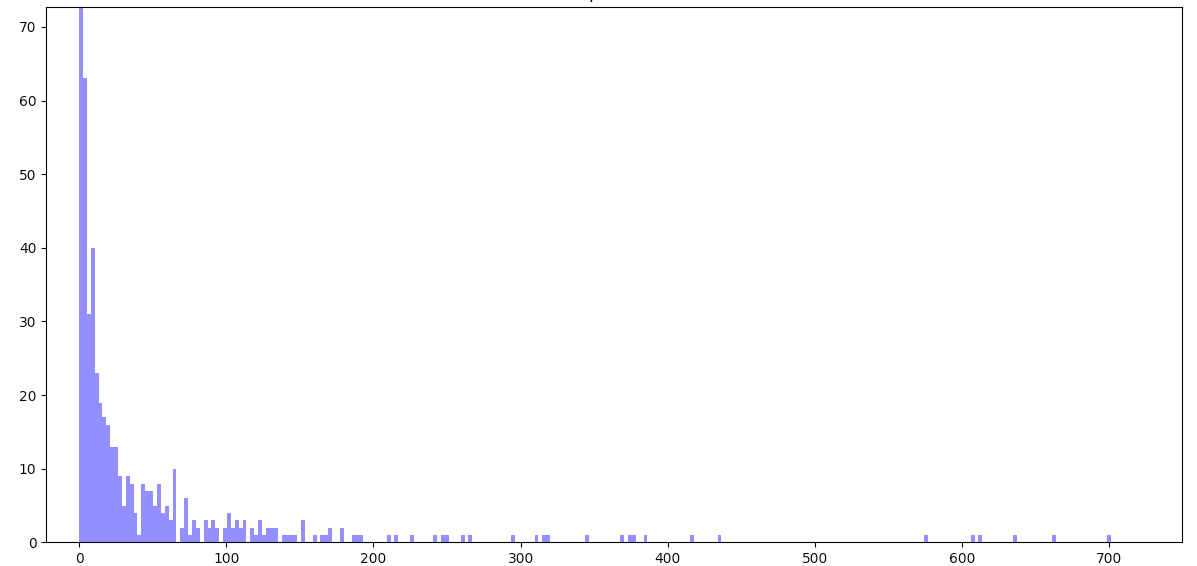
\includegraphics[width=\linewidth]{num_proteins_fold_155}
    \caption{Here is a histogram of the number of proteins per fold for SCOP 2.07. We see that each fold has much more examples than SCOP 1.55. This may allow our model to learn better.}
    \label{numproteinfold2.07}
\end{figure}

We inspect the distribution of the proteins across the different folds. We see that there are much more proteins per fold.

\begin{figure}
    \includegraphics[width=\linewidth]{chainlengths155}
    \caption{Here is a histogram of the protein lengths for SCOP 2.07. We see that 90\% of the proteins have length less than 500}
    \label{chainlength2.07}
\end{figure}

Once again, we inspect the length of the proteins in our dataset.

Similar to the small dataset, we split up 70\% of the dataset for training, 15\% for validation and 15\% for testing. We adjust the sampling of the validation and testing so that a wide range of folds are represented.

\subsubsection{Members of SCOP Classes}

We take a look at the members of the proteins in each of the 7 SCOP classes to understand their composition When looking at the first 4 classes (Fig.\ref{fig:SCOPClass-abcd}) we see that most of the protein in the Alpha, Beta, Alpha/Beta, and Alpha+Beta classes fall in line with their descriptions in the SCOP paper. Alpha proteins consists almost exclusively of alpha helices, beta proteins consist almost exclusively of beta sheets, Alpha/Beta proteins consist of alpha helices and beta sheets very tightly intertwined, and Alpha+Beta proteins consist of alpha helices and beta sheets relatively in separate locations.

\begin{figure*}[t]
\centering
\begin{subfigure}{.5\textwidth}
  \centering
  \includegraphics[width=.7\linewidth]{img/SCOP/aProtein-d1kdxa_}
  \caption{Alpha protein d1kdxa\_}
\end{subfigure}%
\begin{subfigure}{.5\textwidth}
  \centering
  \includegraphics[width=.7\linewidth]{img/SCOP/bProtein-d2giyb2}
  \caption{Beta protein d2giyb2}
\end{subfigure}
\begin{subfigure}{.5\textwidth}
  \centering
  \includegraphics[width=.7\linewidth]{img/SCOP/cProtein-d1btma_}
  \caption{Alpha/Beta protein d1btma\_}
\end{subfigure}%
\begin{subfigure}{.5\textwidth}
  \centering
  \includegraphics[width=.7\linewidth]{img/SCOP/dProtein-d1bc4a_}
  \caption{Alpha+Beta protein d1bc4a\_}
\end{subfigure}%
\caption{Here are sample proteins representative of the first 4 types of SCOP classes. We note that most of the proteins in these classes show clear structural similarity.}
\label{fig:SCOPClass-abcd}
\end{figure*}

When we look at the remaining classes, we see a wider range of topological structures within each class \ref{fig:SCOPClass-efg}. Within the Multi-domain protein class, we see protein d1i99i (Fig.\ref{e1}), which has Alpha Helices and Beta sheets in relatively different locations, and protein d1x75a1 (Fig.\ref{e2}), which consists only of alpha helices. Within the Membrane and cell surface protein and peptide class, we see protein d1uaza\_ (Fig.\ref{f1}) which consists entirely of alpha helices and protein d1m3ia (Fig.\ref{f2}) which consists of alpha helices and beta sheets interspersed throughout the protein. Finally, for the small protein class, we see protein d1ehsa\_ (Fig.\ref{g1}), which is comprised solely of alpha helices and protein d1wj2a\_ (Fig.\ref{g2}). which is comprised solely of beta sheets. Furthermore we note that protein d1i99i (Fig.\ref{e1}) has structural similarity to proteins in Alpha+Beta Class and protein d1x75a1 (Fig.\ref{e2}) has structural similarity to proteins in Alpha Class. These inter-class structural similarities may pose a challenge when trying to classify these proteins accurately.

\begin{figure*}
\centering
\begin{subfigure}{.5\textwidth}
  \centering
  \includegraphics[width=.7\linewidth]{img/SCOP/eProtein-d1i99i_}
  \caption{Multi-domain protein d1i99i\_}
  \label{e1}
\end{subfigure}%
\begin{subfigure}{.5\textwidth}
  \centering
  \includegraphics[width=.7\linewidth]{img/SCOP/eProtein-d1x75a1}
  \caption{Multi-domain protein d1x75a1}
  \label{e2}
\end{subfigure}

\begin{subfigure}{.45\textwidth}
  \centering
  \includegraphics[width=.7\linewidth]{img/SCOP/f1Protein-d1uaza_}
  \caption{Membrane and cell surface protein and peptide d1uaza\_}
  \label{f1}
\end{subfigure}%
\begin{subfigure}{.45\textwidth}
  \centering
  \includegraphics[width=.7\linewidth]{img/SCOP/f2Protein-d1m3ia}
  \caption{Membrane and cell surface protein and peptide d1m3ia}
  \label{f2}
\end{subfigure}%

\begin{subfigure}{.5\textwidth}
  \centering
  \includegraphics[width=.7\linewidth]{img/SCOP/g2Protein-d1ehsa_}
  \caption{Small protein d1ehsa\_}
  \label{g1}
\end{subfigure}%
\begin{subfigure}{.5\textwidth}
  \centering
  \includegraphics[width=.7\linewidth]{img/SCOP/gSmallProtein-d1wj2a_}
  \caption{Small protein d1wj2a\_}
  \label{g2}
\end{subfigure}%
\caption{Here are pairs of very different proteins within each of the last three types of SCOP classes. We note that some of these proteins have structures very similar to some of the proteins in the first four SCOP classes. These variations indicate structural dissimilarity within the last three SCOP classes.}
\label{fig:SCOPClass-efg}
\end{figure*}

%----------------------
\subsection{SCOP Viewer}
%----------------------
A number of tools were developed during the research to help view the data and guide the direction of the research. SCOP Viewer, a tool to visualize protein structure and the navigate through the different barcodes was developed to inspect the output of the protein backbone parse and the homology cycles generated by the persistent homology. The tool allows 3D navigation, allowing much more clarity in understanding more complex structures than a 2D image.

The tool is very flexible for general use, allowing the user to feed in a point cloud and allowing the user to view the generated persistence homology. 

\begin{figure}
    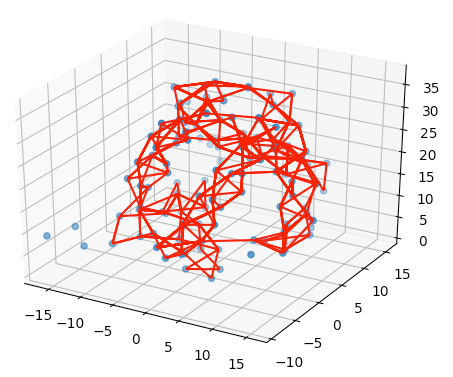
\includegraphics[width=\linewidth]{img/scopviewer/scopviewer1}
    \caption{SCOP Viewer allows the user to view the generated persistence homology of the data at once. Here are the generated cycles of protein 1dly}
    \label{}
\end{figure}

\begin{figure}
    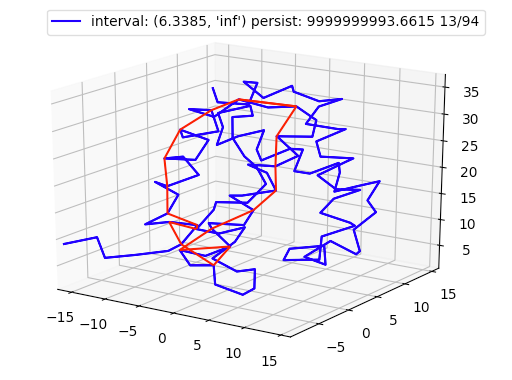
\includegraphics[width=\linewidth]{img/scopviewer/scopviewer2}
    \caption{SCOP Viewer allows the user to cycle between the various types of persistent cycles generated for our protein. Here we have a cycle describing a beta sheet structure for protein 1dly. }
    \label{}
\end{figure}

%----------------------
\subsection{Third Party Tools}
%----------------------
A number of third party tools were used as part of the research. ProDy's (Protein Dynamics \& Sequence Analysis) python package was used to extract the backbone structure from each protein's PDB file. NumPy package was used for matrix  and statistical operations. Matplotlib package was used to generate histograms and 3D plots of the proteins and the barcodes. Pillow was used to generate the 2D images of the distance matrix and the barcode images. Keras and Tensorflow were used to setup and train the convolutional neural network. CPickle package was used to serialize and deserialize processed data.
%---------------------- 
\subsection{Computing Resources}
%----------------------
Initially the research started on a personal laptop without a GPU and very limited storage space [Ref: Table]. Since the unpacked data of SCOPe 2.07 took up around 40GB and the laptop ran out of storage space, the data was stored on a flash drive. 

The lack of a GPU made the training very slow. Even relatively simple methods on the smaller, SCOP 1.55, dataset took around 40 hours. Furthermore, the small storage space made it difficult to unpack and save the processed data on the larger SCOPe 2.07 dataset. These factors significantly slowed the progress of the research.


\begin{table*}[h]
    \centering
    \begin{tabular}{|c | c | c |}
    	\hline
    	                    &  \textbf{Personal Laptop} &  \textbf{Personal Workstation} \\ \hline
        \textbf{CPU} & Intel Core i7-4650U &  E5-2630 6-Core \\ \hline
         \textbf{GPU (CUDA-enabled)} & None & Nvidia GTX 1060 6GB      \\ \hline
         \textbf{RAM} & 8GB & 16GB   \\ \hline
         \textbf{Storage} & 128GB SSD & 500GB SSD \\ \hline
         \textbf{OS} & MacOSx   & Ubuntu 16.02 \\ \hline
    \end{tabular}
    \caption{A comparison of the laptop and the workstation. Purchasing the workstation made possible significant advancements in the research by increasing the speed of computation and also allowing to work with larger datasets. }
    \label{tbl:Computers}
\end{table*}

Due to the limitations of the personal laptop, a personal workstation was purchased at \$500 on Winter of 2018 [Ref: Table]. Although it has modest computing power relative to industry standards, the purchased machine led to significant increases in speed and efficiency of the research. The most important changes in computer resources were the GPU, which led to increases in training speed, and the increased storage, which made it possible to work on the larger SCOPe 2.07 dataset. It is also worth nothing that Ubuntu has better support than MacOSx for running CUDA.
Most of the optimized methods took around 16 hours at most to complete on the large SCOPe 2.07 database, which is 8 times larger than the smaller SCOP 1.55. 


% ===============================================================
\section{Methods}
% ===============================================================

%---------------------
\subsection{ Background Information: Proteins} \label{Background Information: Proteins}
%---------------------
A protein is an sequence of amino acids, a set of 22 compounds which link sequentially into a protein chain. The interaction between amino acids and the surrounding environment determine the how the protein folds into its structure.

For a protein that we are tasked to classify, we are provided with many information: Protein sequence and the sequential coordinates of every atom on our protein. Since we are primarily interested in the topological features of our data, we characterize the protein's shape with the protein backbone. The protein's backbone is constructed with a sequence of points, where each point represents each amino acid in a 3D space. The point representation of each amino acid is determined by the algorithm 'parsePDB' in the ProDy package. 

Since we will be dealing primarily with the protein's backbone, we introduce the following notation.
    
\begin{defn}
A protein, $P$, with sequence of N amino acids will be a called a protein with length N. It's backbone will be denoted as a sequence of 3D coordinate points $ \{P_i\}^{N}_{i=1} $ where $P_{i} \in \mathbb{R}^3 $

For each coordinate point $ P_{i} $, the x-coordinate is referred as $ P_{i}(1) $, y-coordinate as $ P_{i}(2) $, and z-coordinate as $ P_{i}(3) $.
\end{defn}

We extract two distinguishing types of input features from the protein's backbone chain: Distance matrix and Persistence Homology. These two features are very robust. They are both rotation and translation invariant, meaning that the features remain the same even if the protein is rotated or moved. They are also very stable: minor changes to the data does not create a significant variation in the feature.
    
%---------------------
\subsection{ Backbone Chain}
%---------------------  
Each the dataset of proteins are stored as PDB (Protein Data Bank) files, which describe the shape of the 3D protein. The dataset tar [Ref] files unpack into main directory, pdbstyle-1.55 and pdbstyle-2.07 for SCOP 1.55 and SCOPe 2.07 respectively. Each PDB file is stored in a subdirectory under the main directory. The name of the subdirectory is determined by the protein's name.

The index files for SCOP 1.55 and SCOPe 2.07, 'dir.cla.scop.1.55.txt' and 'dir.cla.scope.2.07-stable.txt', provide important information for each protein in our database [Ref: index example]. 

\begin{table*}[h]
    \centering
    \begin{tabular}{| l | l|}
        \hline 
        Index Entry & d1dlwa\_ 1dlw    A:  a.1.1.1 14982	cl=46456,cf=46457 ... \\ \hline
        Name & d1dlwa\_     \\ \hline
        Class.Folds.Superfamily.Family & a.1.1.1    \\ \hline
    \end{tabular}
    \caption{ Here is the relationship between the index entry of a protein and the protein in the dataset. The PDB file for this protein found under the subdirectory 'dl' as 'd1dlwa\_.ent'}
    \label{tbl:Index Entry}
\end{table*}

For each protein, protein backbone chain is parsed from the PDB file using the 'parsePDB' function in the ProDy package. The extracted coordinates of the protein backbone is saved as a list. 

The class and the fold number of the protein uniquely identifies a protein's fold. We create a one to one mapping between class-fold to the integers. These integers are the labels of our protein-fold classification problem.

Because all of the protein coordinates do not fit on the RAM, they are saved in batches of 10000. In each batch, the protein coordinates and the fold labels are saved into a dictionary under the keys b'x' and b'y' respectively.

%---------------------
\subsection{ Distance Matrix}
%---------------------
With the points in the protein backbone, we construct a distance matrix of the distances between the points. The unit of the distances Ångströms, the units of provided in the protein PDB files. [Protein Data Bank]. We used the Euclidean Distance for the distances between the points.\\

    
\begin{defn}
    For a protein $P$ with length N, we denote it's distance as matrix $M_{P}$.
    We construct it as follows.
    $ M_{P} := [M_{ij}] $ where 
    \begin{multline*}
    M_{ij} = Euclidean Distance(P_i, P_j) = \\ \sqrt{P_i(1)-P_j(1))^2+(P_i(2)-P_j(2))^2} \\ +(P_i(3)-P_j(3))^2
    \end{multline*}
\end{defn}

\noindent
\textbf{Remark}\\
We note the following for any distance matrix $M_{P}$.
    \begin{itemize}
        \item $M_{ii} = 0$
        \item $M_{ij} = M_{ji}$
        \item The intersection of the ith row and the jth column corresponds to $M_{ij}$, the distance between the ith and the jth point.
    \end{itemize}
    
\begin{figure}[h]
	\centering
    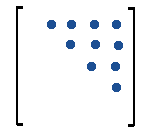
\includegraphics[width=.7\linewidth]{uptry.png}
    \caption{Here we have the entries in a matrix that correspond to the upper triangle. We note that since our distance matrix is symmetric with respect the diagonal line, we only need to calculate the distance values once for the entries in the upper triangle of our matrix.}
     \ref{uptry}
    \label{uptry}
\end{figure}
    

We see that the distance matrix is symmetric (Fig.\ref{uptry}) since the distance between the ith and the jth point is the same as the distance between the jth point and the ith point. Because of this, we only need to compute the distance between these pairs of points once. Also, the distance between a point to itself is zero. So the pairs of ith and jth's points we need to compute the distances for lie in the upper triangular region of the distance matrix. This region is consists of $\{ M_{ij} \space | \space i<j \}$ [Ref:]. Computing the distance matrix in this fashion divides the computation time by about half. Because the distance matrices of the entire dataset are larger than the size of the RAM, the data is split up into 1000 sized batches. 

\begin{algorithm}
\caption{We fill in our distance matrix by calculating the upper triangle of a NxN matrix. Our rows and columns range from 1 to N.}
\begin{algorithmic}
\STATE{M is distance matrix set with zeroes}
\STATE{Euclid(a,b) is the distance between a and b}
\FOR{r <= N}
    \FOR{c < r}
    	\STATE{d=Euclid(r,c)}
        \STATE{M(r,c)=d}
        \STATE{M(c,r)=d}
    \ENDFOR
\ENDFOR
\end{algorithmic}
\end{algorithm}

\begin{figure}[H]
	\centering
    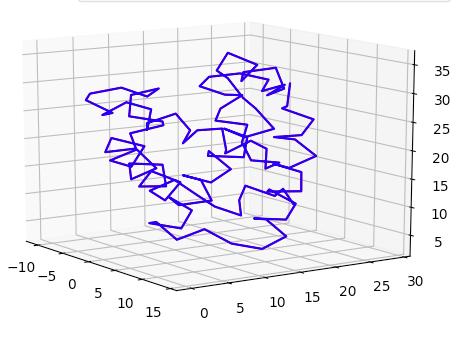
\includegraphics[width=\linewidth]{1ux8pdb.png}
    \caption{Here is the 3D shape of the  1ux8 protein's backbone chain. We see that there are notable features, alpha helices and beta sheets, that we would like to represent in our distance matrix.}
    \label{1ux8pdb}
\end{figure}

We inspect the topological structure of our protein '1ux8'. It is a protein of length 118. This protein has some spiral structures (alpha helix). These spiral structures sometimes lie in close promixity in parallel or anti parallel direction (beta sheet). These types of structures (secondary structures) are known in molecular biology to be important features of a protein's shape.

\begin{figure}[H]
    \centering
    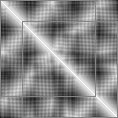
\includegraphics[width=\linewidth]{1ux8matBase}
    \caption{Here is the distance matrix of the 1ux8 protein. We see a thick diagonal line with corresponds to the protein backbone chain.}
    \label{1ux8matBase}
\end{figure}
    
We analyze the distance matrix to see if important structural features are represented in the matrix. To help with visualization, the distance matrix is mapped to an image of equal size, where closest distances appear in white and furthest distances appear in black. Distances in between take a gray hue with the intensity based on its value.
\\

\noindent
\textbf{Feature Protein Backbone:}\\
Along the diagonal line of the image, the distance matrix is completely white. This is because the distance between a point to itself is zero [Ref: Remark]. We note that this diagonal white line uniquely identifies the protein backbone chain (Since the distance between. Having a clear representation of the protein backbone is important because  it is a central structure that other features can be spatially oriented around.
\\

\noindent
\textbf{Feature Alpha Helix:}\\
We note thick white regions running parallel along the diagonal line of the image [Ref: Image]. These regions indicate that at a given point in the chain, it is in close proximity to the nearby neighbors [Ref Diagram]. We also note that in for a point in an Alpha Helix, it is also in close proximity to it's nearby neighbors. In our example, these four thick white regions correspond the the four helix structures on our protein.
    
\begin{figure}[h]
    \centering
    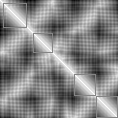
\includegraphics[width=\linewidth]{1ux8matAhelix}
    \caption{The red squares outline the discrete thick white regions running parrallel to the diagonal line. These regions indicate that the neighbors of points in this region are in very close proximity, indicating that there may be a helix. }
    \label{1ux8matAhelix}
\end{figure}

    
\begin{figure}[h]
    \centering
    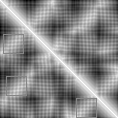
\includegraphics[width=\linewidth]{1ux8matBetaSheets}
    \caption{The blue squares outline the lines of proximity between points on different helicies, suggesting that the helices are in close proximity. The direction of the lines indicate whether the two helices are parallel or anti-parallel.}
    \label{1ux8matBetaSheets}
\end{figure}

\begin{defn}
A helix is composed of points in the protein backbone. Suppose $H$ is the set of indices of these points along the length of the protein. We call the row belonging to this helix as the collection of rows, $R_{i}$, of the distance matrix such that the rows contain elements of the helix. $\{R_{i} \space | \space i \in H \}$. Similarly we define the column belonging to the helix as $\{C_{i} \space | \space i \in H \}$.
\end{defn}

\noindent
\textbf{Feature Beta Sheet:}\\
We note patches of thick white lines in the intersection of the rows belonging to a helix and the columns belonging to another helix [Ref Diagram]. This indicates that the points of the two helices, and hence the two helices, are in close proximity. In particular, the regions are close sequentially: the ith point in helix A is close to the jth point in helix B and the i+1 th point in helix A is close to the j-1 th point in helix B. This sequential relationship describes a Anti-parallel Beta Sheets. For Parallel Beta Sheets, the i+1 th point would be close to the j+1 th point. In our example, the 3 pairs of Beta-sheets formed the 4 helices are represented in our distance matrix.
%----------------------    
\subsubsection{ Cropped Distance Matrix}
%----------------------
Some proteins have a length of 600, making the distance matrix have a size of 600x600. However, due limitations on the GPU memory, it is not possible to construct a convolutional network with our input being 600x600. We would also like to crop the distance matrix such that the central backbone of the protein runs through the diagonal of our matrix. To crop and preserve the diagonal protein backbone, we take a 100x100 window and crop our matrix by shifting row and columns at the same time by 50 indices.

\begin{figure}[h]
    \centering
    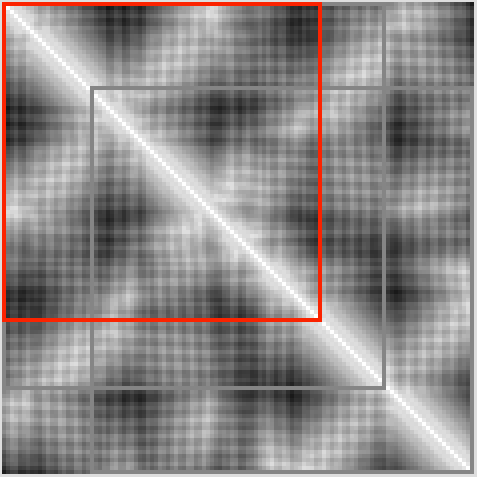
\includegraphics[width=\linewidth]{cropMat}
    \caption{Due to computational restrictions, we crop our matrix by shifting the red crop window along the diagonal line of our matrix.}
    \label{cropMat}
\end{figure}

Because of the limitations set by the windowed distance matrix, a point in the backbone can only see information about, on average, half of the window size forwards and backwards. This limitation affects the cropped matrix's ability to detect longer range contact information, which can be critical in determining the protein's overall shape. In our example [Ref], the cropped distance matrix would not see information about the proximity between the first alpha helix and the third alpha helix because they are too far away in the backbone index.

\begin{figure}[h]
    \centering
    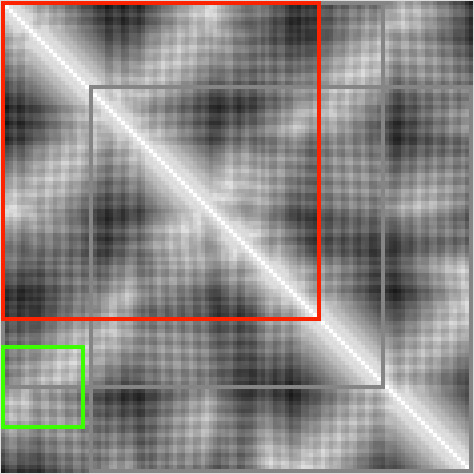
\includegraphics[width=\linewidth]{cropMatMiss}
    \caption{We note that cropping the distance matrix may cause a loss of long range contact information. In our protein 1ux8, the cropped matrices do not detect that the alpha helix 1 forms a beta sheet with alpha helix 3}
    \label{cropMatMiss}
\end{figure}

We note that if a distance matrix is smaller than our cropping window size, we pad the distance matrix.

Cropping the dataset increases the number of examples in the dataset. Because we don't want our training data to have similarities, we make sure that the training, validation, and testing groups do not share cropped matrices from the same protein.
%----------------------
\subsubsection{ Sparse Distance Matrix}
%----------------------
In our example, we see that cropping the distance matrix diminishes it's ability to represent long range contact information. We develop an alternative approach to reduce the size of the distance matrix while preserving it's ability to represent long range contact information.

\begin{figure}[h]
    \centering
    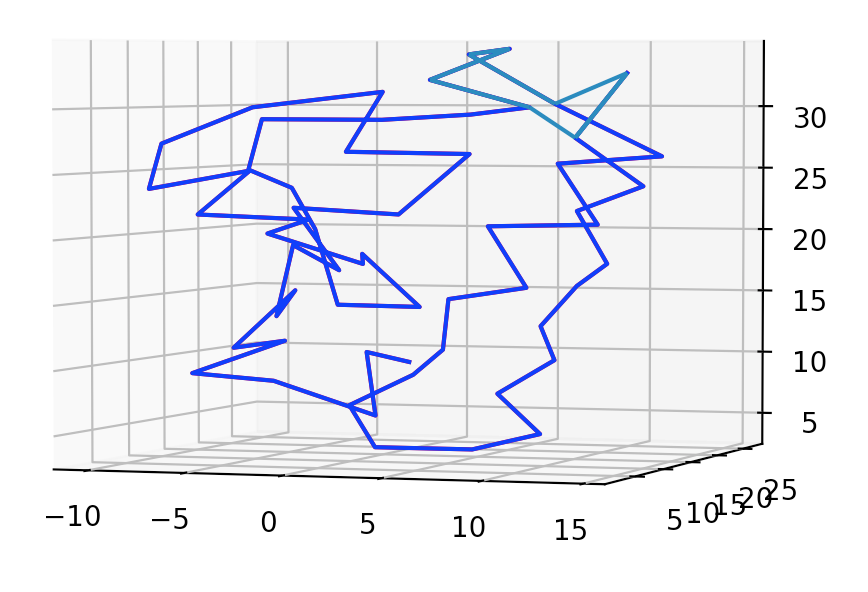
\includegraphics[width=\linewidth]{1ux8sparse}
    \caption{Due to computation restrictions, we sample every other point on our protein and compare it with the original structure. We see that, although diminished, most of the features of the protein are still distinguishable.}
    \label{1ux8sparse}
\end{figure}

Given, a protein backbone with length N, $\{P_i\}^{N}_{i=1}$, we sample every other point, $\{P_i \space | \space \text{i is odd} \}$, to create a sparse protein backbone. We graph the sparse protein backbone in 3D space [Ref ] and compare it to the original protein backbone [Ref: Original Chain]. In comparison, we see that the general structure of the protein and its features are diminished but preserved.

\begin{figure}[h]
    \centering
    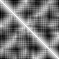
\includegraphics[width=\linewidth]{1ux8pdbSparseDistM}
    \caption{Here we have a distance matrix of the sampled 1ux8 protein backbone. We do see that the protein backbone, alpha helices, and beta sheets that were observed in the full distance matrix can also be observed in the sparse distance matrix. }
    \label{1ux8pdbSparseDistM}
\end{figure}

From the sparse protein backbone, we construct a sparse distance matrix in the same fashion as a regular distance matrix. In example, we compare the sparse distance matrix [Ref:] and the unmodified distance matrix [Ref:] and see if the backbone chain, alpha helix and beta sheet features are preserved in the distance matrix. First, we see that the diagonal backbone is preserved in the matrix. Second, we do see that the alpha helix features are preserved, even though it is less clearly defined. Finally, we see that the beta sheet features are preserved as well.

For the protein of length 600, the sparse distance matrix would reduce the matrix's size from 600x600 to 300x300. This is still too big for due to the limitations on the GPU memory. So we crop the sparse distance matrix in the same manner as a regular distance matrix. We also take care such that the training, validation, and testing groups do not share cropped matrices from the same protein.



%---------------------
\subsection{ Persistent Homology}
%---------------------
\textbf{Persistent Homology: } Topological data analysis is applied to the points in the protein backbone to produce persistent barcodes. The barcodes indicate when simplexes are formed and are destroyed. Significant topological features of the data are represented by these barcodes.


\subsubsection{ Mathematical Background}

A good deal of effort went into trying to make the mathematical definitions used this section self-contained. One could read through this section to get a general understanding of the theory behind persistence homology. However, there are some fundamental concepts in abstract and linear algebra that were not defined. These are, but not limited to the following: group, normal subgroup, quotient group, homomorphism, kernel, image, vector space, dimension of a vector space.

We discuss the mathematical theory behind persistent homology prior to introducing an algorithm to compute it.  First, we describe the elementary mathematical objects. Then we describe the topological features of a data that we want to extract using the homology and the structure theorem. We also discuss the stability of the topological features described by the stability theorem.

\begin{figure}[t]
\centering
    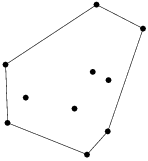
\includegraphics[width=.6\linewidth]{img/mathDef/ConvexHull2D}
    \caption{Illustration of a convex hull of 10 points. For a finite set of points this is just a a polygon connecting the outer most points.}
    \label{ConvexHull}
\end{figure}

\begin{defn}
A \textbf{convex set}, $C \subset \mathbb{R}^n$, is a set where $\forall a,b \in C$, $t \in [0,1]$ $ta+(1-t)b \in C$.
\end{defn}

\begin{defn}
A \textbf{convex hull} $<A>$ of a set of points, $A \subset \mathbb{R}^n$ is defined by 
$$<A> := \bigcap \{C \mid C \text{ convex in } \mathbb{R}^n \text{ , } A\subset C \} $$
\end{defn}

\begin{figure}[t]
    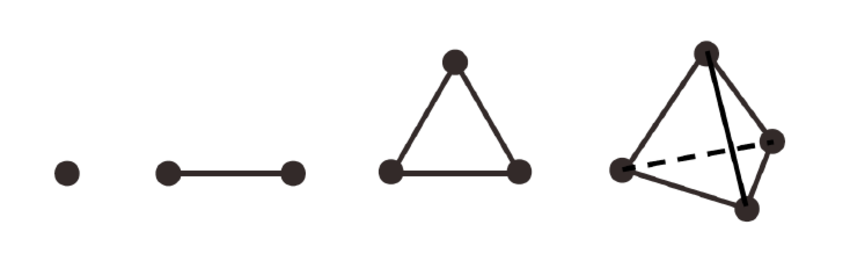
\includegraphics[width=\linewidth]{img/mathDef/simplex.png}
    \caption{Here are illustrations of a 0-Simplex (a point), 1-Simplex (a line), 2-Simplex (a triangle), 3-Simplex (a tetrahedron)}
    \label{Simplex}
\end{figure}

\begin{defn}
An \textbf{$n$-simplex} is a convex hull of $n+1$ points. When we refer to varying sizes n-simplices together or when the size is undetermined, we will call them just simplex/simplices.\\
We note that $0$-simplex is a point, $1$-simplex is an edge, and $2$-simplex is a trangle.
\end{defn}

\begin{defn}
Let $\sigma$ be a simplex.
\begin{itemize}
\item The \textbf{vertices} of $\sigma$ are its points.
\item The \textbf{face} of $\sigma$ are the simplices formed by subset of the vertices of $\sigma$.
\item A  \textbf{n-face} is a face of $\sigma$ with $n+1$ vertices.
\end{itemize}
\end{defn}

\begin{defn}
\textbf{Simplicial complex} is a set of simplices, $S $, such that 
\begin{itemize}
    \item Any face of a simplex $\sigma \in S$ is in $S$.
    \item The intersection of any two simplices in $ S $ is in $ S $
\end{itemize}
\end{defn}

\begin{figure}[t]
    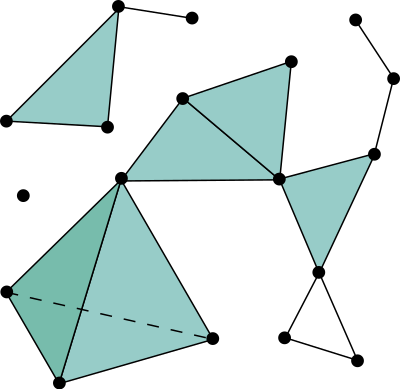
\includegraphics[width=\linewidth]{img/mathDef/simpcomplex}
    \caption{Here is an illustration of a simplicial complex. Notice that it is a collection of points,edges and triangles.}
    \label{simpcomplex}
\end{figure}

Now that we have defined the foundational definitions, we begin to define structures that can describe the topological characteristics of the points in a protein's backbone. First, we will observe the structure of our protein as we create simplices by adding edges of increasing length between the points on the protein's backbone. We do this by forming Vietoris-Rips complexes.

\begin{defn}
Given a set of points with a metric, a \textbf{$\epsilon$-Vietoris-Rips complex} on the set of points is a simplicial complex which is formed by connecting the points with distance less than or equal to $\epsilon$.
\end{defn}


\begin{figure}[t]
    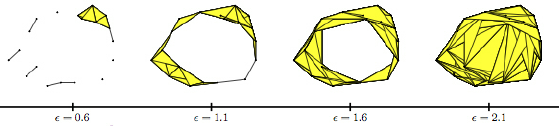
\includegraphics[width=\linewidth]{img/mathDef/ripscomplex.png}
    \caption{Here is a series of 5 Vietoris-Rips complexes. At $\epsilon=0$ we only have a collection of points, while at $\epsilon=1.1$ we being to see an interesting characteristic of our data beginning to form. Finally, at $\epsilon=2.1$ we do not see much of a structure as most of the points become interconnected to each other. }
    \label{}
\end{figure}

First, we create $\epsilon$-Vietoris-Rips complexes of our points in the protein backbone for all intervals of $\epsilon$. We see how the state of our data changes as we add edges between points of increasing length by ordering the $\epsilon$-Vietoris-Rips complexes in increasing order of $\epsilon$. This ordering is a filtration on the set of all Vietoris-Rips complexes on our data. If $\epsilon_1 \leq \epsilon_2$ then $\epsilon_1$-Vietoris-Rips complex is contained in  $\epsilon_2$-Vietoris-Rips complex. This is because edges less than $\epsilon_1$ are also less than $\epsilon_2$ and thus are formed in  $\epsilon_2$-Vietoris-Rips complex.

\begin{defn}
\textbf{A filtration} is an ordering on $S_i \in \mathbb{S}$ such that
$$S_1 \subseteq S_2 \subseteq S_3 \subseteq S_4 \subseteq ...$$.
\end{defn}

We denote $\epsilon$-Vietoris-Rips complexes as $V_{\epsilon}$ and write our filtration of $V_{\epsilon}$s.


 $$V_{\epsilon_1}\subseteq V_{\epsilon_2} \subseteq V_{\epsilon_3} \subseteq V_{\epsilon_4} \subseteq ...$$
 
For each $V_{\epsilon}$, we convert it to an algebraic vector space to allow us to detect holes and other topological features in our simplicial complex. We say we apply a homology on $V_{\epsilon}$. We will define the building blocks prior to defining the homology on a simplicial complex.

\begin{defn}
The group of \textbf{$k$-Chain} of $S$ is an abelian group of elements consisting of 
$$\sum z_i s_i $$ where $z_i \in \mathbb{Z}$ and $s_i$ is a $k$-simplex of S.
$C_k$ is also a vector space.
\end{defn}

\begin{defn}
The \textbf{boundary operator} $\partial_k : C_k \rightarrow C_{k-1}$ is a homeomorphism defined as
$$\partial ([v_1,v_2,...,v_k]) := \sum_{i=0}^{k} (-1)^i [v_1,...,\hat{v_i}, ...,v_k]$$
where $[v_1,...,\hat{v_i}, ...,v_k]$ is a simplex of all elements $v_1$ to $v_k$ except $v_i$.\\
Since we are working with points in $\mathbb{R}^3$, we define the boundary operators that we will use.
$$\partial_1 ([ab]) := b-a$$
$$\partial_2 ([abc]) := ab-ac+bc$$
\end{defn}

\begin{lem}
$\partial_i \circ \partial_{i+1} = 0 $.\\
In other words, the composition of two subsequent boundary functions is zero.\\
\end{lem}

The above lemma implies that $Im \partial_j+1 \subset Ker \partial _j$. Since every subgroup of a normal subgroup is normal and $Ker \partial _j$ is a normal subgroup, we can form the quotient group $\dfrac{Ker \partial _j}{Im \partial_{j+1}}$.


\begin{defn}
Given a simplicial complex, $S$, it's \textbf{j-homology} is the algebraic quotient group, $\dfrac{Ker \partial _j}{Im \partial_{j+1}}$,\\
with the boundary functions are defined on the chain of $S$\\
We denote the j-homology of $S$ as $H_j(S)$\\
We note that the homology is a vector space since $Z_j \subset C_j$ was a vector space.
\end{defn}

We note that the Homology of $S$ is nonzero if $Ker \partial _j \neq Im \partial_{j+1}$. For $H_1$ this means $H_1(S)$ is nonzero if any linear combination of boundaries of triangular simplices in $S$ is not equal to the hole formed by the edges in $S$. In an example with 6 points (Fig.\ref{homHex}), we see that the $H_1$ of the simplex is nonzero because the hole created by the edges $abcd$ is not the linear combinations of the 2 triangular simplices' boundaries, $ebf$ and $dhg$.

The dimension of the homology of a simplicial complex tells us how many holes there are in the simplicial complex.

\begin{figure}
    \includegraphics[width=\linewidth]{img/hom/homologyHex}
    \caption{The homology of this simplicial complex consisting of 6 points is not zero because the hole (blue) created by the $abcd$ edges in the simplex is not equal to the linear combinations of the 2 triangular simplices'  boundaries (red) }
    \label{homHex}
\end{figure}

So far, we can look at the homology of each $V_{\epsilon}$ individually and can tell how many holes are in each simplicial complex. However, homology does not tell use what the holes are. We now move towards trying to utilize the information from homology for all the  $V_{\epsilon}$s.

For each $V_{\epsilon}$ in our filtration, we apply a homology. For our research, we apply a 1-homology, $H_1$, to each of the $V_{\epsilon}$s. The inclusion maps between the subsequent homologies induce a sequence of homomorphisms. This sequence for a given filtration is called the persistence module.
 
 $$ H_1(V_{\epsilon_1}) \rightarrow H_1(V_{\epsilon_2}) \rightarrow H_1(V_{\epsilon_3}) \rightarrow H_1(V_{\epsilon_4}) ...$$
 
\begin{defn}
Given a filtration of simplicial complexes, $S_1 \subseteq S_2 \subseteq S_3 \subseteq S_4 \subseteq ...$, the chain of homologies linked by the homomorphism induced by the inclusion map is called the \textbf{persistence module}, $ H_i(S_1) \rightarrow H_i(S_2) \rightarrow H_i(S_3) \rightarrow H_i(S_4) \rightarrow ...$.
\end{defn}
 
From the results of the structure theorem for persistence homology theory, we can decompose the persistence module into sums of 1 dimensional intervals. In the following example, we can reduce the persistence module for the simplicial complexes 4 points into two intervals.

\begin{figure}[H]
    \includegraphics[width=\linewidth]{img/hom/sqfilt}
    \label{sqfilt}
\end{figure}
 $ H_i(S_1) \rightarrow H_i(S_2) \rightarrow H_i(S_3) \rightarrow H_i(S_4)$\\
 $\simeq \ \ \ \   0 \ \ \  \rightarrow \ \ \ \ \mathbb{R} \ \ \ \rightarrow \ \ \ \  \mathbb{R} \ \ \rightarrow \ \ \ \ \mathbb{R}$\\
 $\oplus \ \ \ \ \ 0 \ \ \ \rightarrow \ \ \ \ 0 \ \ \ \rightarrow \ \ \ \  \mathbb{R} \ \ \ \rightarrow \ \ \ \ 0$\\
 
 The top summand corresponds to the upper triangular hole and is non zero from $ H_i(S_2) $ to $ H_i(S_4) $ because this hole persists through $S_1$ to $S_4$. The bottom summand corresponds to the lower triangular hole and is nonzero only at $ H_i(S_3) $ since this hole is formed at $ S_3 $ and dies at $S_4$. We call summands of this form, where there is a single linked chain of $\mathbb{R}$ ,\textbf{intervals}. These intervals form the barcode that tell us the birth and the death of each hole.

We briefly mention a series of theorems that guarantee that we can decompose any persistence modules into a sum of intervals as we did  in our previous example. These theorems are referred to as structure theorems of persistence homology.

\begin{thm}
A persistence module is indecomposible if and only if it is an interval.
\end{thm}

\begin{thm}
A vector space is indecomposible if and only if it is 1 dimensional.
\end{thm}

\begin{thm}
Any persistence module is a finite sum of indecomposible subgroups.
\end{thm}

\begin{thm}
\textbf{(Krull-Schmidt)} The decomposition of a persistence module is written uniquely as as a sum of indecomposible subgroups. 
\end{thm}

The previous four theorems give us the following. Any persistent module can be written uniquely as a sum of intervals. The result we have now is that given any set of points, we can construct a filtration such that we get a unique barcode that gives us a structural characterization of the points. We now give a formal definition of the barcode for persistence homology on filtrations of $\epsilon$-Vietoris-Rips Complexes.

\begin{defn}
Given a persistence module $P = \oplus_{i=1}^{n} \ Interval_i$, the \textbf{barcode} of thie persistece module is 
$$\{(birth_i,death_i) \mid 1 \leq i \leq n \}$$
- $birth_i$ is the $\epsilon$ value of the $V_{\epsilon}$ corresponding to the first nonzero element in the chain of $Interval$\\
- $death_i$ is the $\epsilon$ value of the $V_{\epsilon}$ corresponding to the last nonzero element in the chain of $Interval$\\
\end{defn}

Supposed we had two sets of points that were similar. They would generate very similar filtrations of simplicial complexes. We would hope that these filtrations have similar barcodes. We first define a metric on two barcodes.

\begin{defn}
Given, two barcodes $X$ \& $Y$, the \textbf{bottleneck distance}, $W_{\infty}(X,Y)$ is
$$ W_{\infty}(X,Y) := \inf_{\phi:X \rightarrow Y} sup_{x \in X} || x - \phi(x)||_{\infty}$$
\end{defn}

The stability theorem states gives us an upper bound for the bottleneck distance between two filtrations of simplicial complexes. Thus that a small differences  between sets of points lead to small differences in the generated filtrations of simplicial complexes. This in turn leads to a small difference between the barcodes. 

In addition to stability of the barcodes, we note that barcodes are translation and rotation invariant features of a point cloud. This is because the barcodes are formed from the filtrations of $\epsilon$-Vietoris-Rips complexes, which generated by the distances between the points. Since the distances between the points are translation and rotation invariant, our barcodes are also translation and rotation invariant.

The stability and translation and rotation invariance of the barcodes make it an excellent feature for machine learning.

\subsubsection{Computation Algorithm}
We describe our implementation of the persistent homology, in addition to variations to the method to improve performance and collect more protein specific simplices. 
In practice, we will use the N points of a protein backbone in this algorithm but for illustrative purposes, we consider a simple collection of N points in the $\mathbb{R}^2$. (Fig.\ref{Collection of points}) Because we are looking at the distances between our points, the method performs exactly the same in $\mathbb{R}^3$ or with any collection of objects with a well defined metric.

\begin{figure}
    \includegraphics[width=\linewidth]{img/homex/points}
    \caption{Here is the collection of the 17 points we are considering in 2D. Although our protein is in 3D, the persistence homology is concerned with the distances between points, allowing in to work for points in any dimension as long as there is a well-defined metric.}
    \label{Collection of points}
\end{figure}

\begin{defn}
We call the (i,j) edge the edge constructed by connecting the ith and the jth point in our set of N points.
\end{defn}

A distance matrix of the our points is calculated. We collect the upper triangular elements of the distance matrix to get the unique edges of our points (unique disregarding direction, making (i,j) edge equal to (j,i) edge). These edges are sorted by length.

\begin{figure}
    \includegraphics[width=\linewidth]{img/homex/distm.png}
    \caption{Here is a distance matrix of our set of 17 points. We will only consider the edges in the upper triangular matrix, because the (i,j) edge represents the same line as the (j,i) edge}
    \label{Distance matrix of example}
\end{figure}

Consider a protein with length 300. The total number of edges for a protein of length 300 is $\sum_{n=1}^{299} n =44851$. The total number of triangular simplices formed by these edges $\binom{300}{3}=\dfrac{300!}{3!297!}=4455100$.  We see that the numbers of triangular simplices increase exponentially and very quickly, even for small structures. This demands a need to reduce the computation load.

A cutoff distance is determined, where we discard the edges that are larger than this value. A similar concept exists in bioinformatics, where a point of a protein are determined to be in contact with another point if their distance is within the contact distance (3 Å). The loss of information by discarding the edges larger than this value isn't an issue since because when we start considering larger edges, we start converging towards a structure where every point is connected to each other. As long as we set the cutoff distance at an appropriate value, we would still get the cycles of the protein that represent the characteristic features. Furthermore, setting of a cutoff distance has an added advantage that it filters out uninteresting cycles that are too large. We experimentally determined the cutoff distance at 6.5 Å, because 6 Å is the approximate distances between two alpha helices in a beta sheet \cite{fastSCOP}. The distance between two alpha helices are less than 6.5  Å, we  consider the edges that link two alpha helices together, allowing use to extract features related to the beta sheets. Furthermore, the most sequential distances between the backbone points, $P_i and P_{i+1}$, and the distances within the alpha helices are both less than 6.5, allowing use to extract features related to them as well. It is also know that due to   tetrahedral chemical bonding at the carbon backbone atom due to the pleated appearance of beta-strand causes the distance between beta sheets to be approximately 6 Å \cite{fastSCOP}.

For our set of 17 points, the cutoff distance is determined as $\dfrac{1}{6}$ of the longest length, which is around 2. Below are the collection of points 

\begin{figure*}
    \includegraphics[width=\linewidth]{img/homex/cutoff.png}
    \caption{Here we see the effect of the cutoff distance on the triangular simplicies we form. When a cutoff distance is not set ($\epsilon=\infty$), all the edges are considered, forming triangular simplicies where every point is connected to each other. These simplices don't convey too much about the structure of our protein. When a cutoff distance is set properly ($\epsilon=2$), the important distances considered, making the simplices less convoluted and increasing computation time.}
    \label{Effect of cutoff}
\end{figure*}

Once we have the edges that we are considering, we find the triangular simplicies formed by our edges. As we loop over the edges, we index the edges from 1 to N based on the endpoints of the edge (For an edge (2,4),   it is indexed as 2 and 4). Then, we check if each edge forms a triangular simplicies by looking at the indexed edges related to our edge. (For an edge (2,4), we look at the edges that have been index as 2 or 4 to see if we formed a 2-simplex). Because we are forming the triangular simplicies as we add increasing edges, triangular simplicies are ordered by when they are created. 

\begin{algorithm}
\caption{Finding triangular simplicies formed by the edges}
\begin{algorithmic}
\FOR{(i,j) in Edges}
    \FOR{edges indexed i and indexed j}
        \STATE{See if these edges form a triangular simplicies with (i,j)}
    \ENDFOR
    \STATE{Index (i,j) as i and j}
\ENDFOR
\end{algorithmic}
\end{algorithm}

Given a triangular simplex, we can compute when it was born by looking at it's edges. For example, a triangular simplex (1,2,3) has the edges (1,2), (1,3), and (3,1). Suppose the lengths of these edges were 3,5, and 7 respectively. Then the triangular simplex was formed at radius 7. 

\begin{figure*}
    \includegraphics[width=\linewidth]{img/homex/ripcomplex.png}
    \caption{The triangular simplices are discovered as we add edges. Because we are adding the edges in increasing order, the triangular simplices are discovered in the order of their birth.}
    \label{Simplex formation algorithm}
\end{figure*}

From the edges and triangular simplices, we create two matrices, D1 and D2. Let M be the number of edges we are considering and L be the number of triangular simplices we are considering.

D1 is a  NxM matrix where the rows correspond to the backbone points and the columns corresponds to the edge in increasing order. We fill in D1 in the following order. For the hth  edge with endpoints (i,j), we set $D1_{h,i} = -1$ and $D1_{h,j} = 1$. Suppose an edge (2,4) is the 10th smallest edge. The corresponding entries in would be $D1_{10,2}=-1$ and $D1_{10,4}=1$.

\begin{algorithm}
\caption{Constructing D1}
\begin{algorithmic}
\FOR{hth edge (i,j) in Edges}
    \STATE{$D1_{h,i} = -1$}
    \STATE{$D1_{h,j} = 1$}
\ENDFOR
\end{algorithmic}
\end{algorithm}

D2 is a MxL matrix where the rows correspond the edges in increasing order and the columns correspond to the triangular simplicies in created order. We fill in D2 in the following order. For the hth triangular simplex with endpoint (i,j,k), we set $D2_{h,i} = 1$, $D2_{h,j} = 1$ , and $D2_{h,k} = -1$. Suppose an edge (2,4,9) is the 10th triangular simplex. The corresponding entries in would be $D2_{10,2}=1$, $D2_{10,4}=1$, and $D2_{10,9}=-1$. 

\begin{algorithm}
\caption{Constructing D2}
\begin{algorithmic}
\FOR{hth edge (i,j,k) in Edges}
    \STATE{$D2_{h,i} = 1$}
    \STATE{$D2_{h,j} = 1$}
     \STATE{$D2_{h,k} = -1$}
\ENDFOR
\end{algorithmic}
\end{algorithm}

Each of the matrices, D1 and D2, are reduced to echelon form with the following algorithm. A pivot at a given column is given by the last nonzero entry in the column. We try to make all the columns not share any pivots. We loop over the columns and set check if the previous columns share a pivot with the current column. If they share a pivot, a multiple of the sharing pivot is subtracted from the current pivot such that the they do not share pivots. This process is repeated until the current column does not share a pivot with any of the previous columns. Every time the matrix is modified the same operation is performed to an identity matrix, MxM identity matrix for D1 and LxL identity matrix for D2. After we finish reducing the matrix, we call the reduced matrix R1 and R2 and the corresponding modified identity matrices V1 and V2.

\begin{algorithm}
\caption{Reduction of a matrix}
\begin{algorithmic}
\FOR{column in Columns of D2}
    \FOR{pcolumn in Columns before column}
        \IF{column share the same pivot as pcolumn} 
            \STATE{k=$\dfrac{column[pivot]}{pcolumn[pivot]}$}
            \STATE{column -= k*pcolumn}
        \ENDIF
    \ENDFOR 
\ENDFOR
\end{algorithmic}
\end{algorithm}

Finally, we can construct the main matrix that gives us the persistence homology of our protein. First we construct matrix B from the nonzero columns of matrix R2.  Second we construct matrix Z from columns of V1 corresponding to zero columns of R1. The main matrix is then constructed by taking matrix B and appending columns from matrix Z which do not share pivots with columns of our main matrix until the total number of columns is equal to the number of columns in matrix Z.

\begin{algorithm}
\caption{Construction of Main Matrix}
\begin{algorithmic}
\STATE {Main = B}
\FOR{column in Columns of Z}
    \IF{number of columns in Main equals number of columns in Z}
        \STATE{Exit Loop}
    \ENDIF
    \IF{column doesn't share pivots with columns of Main}   
        \STATE{Append column to Main}
    \ENDIF
\ENDFOR
\end{algorithmic}
\end{algorithm}

\begin{figure*}
    \includegraphics[width=\linewidth]{img/homex/matProcess.png}
    \caption{Here we have a diagram of the matrices that we have constructed and manipulated. The final product, the main matrix, is a MxH matrix where M is the number of edges we have considered and H is the simplex with persistent homology.}
    \label{MatricesOfComputeHom}
\end{figure*}

The columns in the main matrix which come from B correspond to the simplices which get created and filled in before our cutoff distance. The columns in the main matrix which come from Z correspond to the simplices that get created but not filled in before our cutoff distance.

From each column,we extract information about the edges that form the simplex and it's birth and death from the column in the following manner. For each column, the simplex is formed by the edges in the non-zero entries in the rows. The simplex is born when the edge corresponding to the last non-zero row is added. If our column comes from B, let d be the column of R2 that our column comes from. Then, the simplex is destroyed/filled in when the dth simplex is formed. If the column comes from Z, then the simplex is not destroyed within our cutoff distance. We notate this by denoting the death as $\infty$. We say that the simplex persists for $death - birth$.

We look at a column of the main matrix which for our example with 17 points.The column is all zero except at rows 13,45,46,50 where it takes the values 1,1,-1,1 respectively, The indices of the non zero the rows correspond the indices of the edges that belong to the hole/cycle. The values 1 and -1 correspond to the orientation of the edge. The longest edge of the hole tells us when the hole was formed. The death of the simplex occurs when the longest edge of the simplexes which fill in our hole is created. This hole/cycle corresponds to the smallest hole found in our data (Fig.\ref{homHoles}). This hole does not persist for a long time, indicating that it is not a significant feature in our data.

We look at another column of the main matrix for our example with 17 points.The column is all zero except at rows 8,9,10,11,13,14,20,22,25,27,31 where it takes the values 1,1,1,-1,-1,1,1,1,-1,-1 respectively. This hole/cycle corresponds to the largest hole found in our data with 11 points (Fig.\ref{homHoles}). This hole persists for a long time, indicating that it is a significant feature in our data.

\begin{figure*}[t]
	\centering
    \includegraphics[width=\linewidth]{img/homex/homHoles}
    \caption{Here we have the 3 holes generated for our example with 17 points. These holes are representative of the features in the data. We see that the first two holes do not persist for a long time, making them less significant feature of the data than the last hole, which persists for a long time.}
    \label{homHoles}
\end{figure*}
\pagebreak

\subsubsection{Persistence Homology Example}

We introduced the theory behind persistence homology and the algorithm to compute it for a set of points. Now we apply persistence homology to our data set. We will first generate the barcode for a protein 1ux8 and see if the backbone chain, alpha helices, and betasheets are represented in the barcodes. We will also compare the features generated by persistence homology and the distance matrix.

We inspect holes generated by persistence homology of our protein 1ux8, a protein of length 118. At each point on the protein backbone, we search an $\epsilon$-radius around the point to connect edges of increasing length to form the $\epsilon$-Vietoris-Rips complexes. Below are a series of $\epsilon$-Vietoris-Rips complexes.

\begin{figure}[H]
    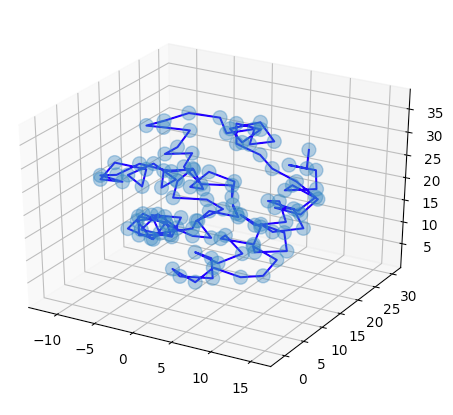
\includegraphics[width=\linewidth]{img/hom/ballRad1.png}
    \caption{$\epsilon = 1$ A search is done at each point at increasing radii to connect the nearby points }
    \label{ballRad1}
\end{figure}


\begin{figure}[H]
    \includegraphics[width=\linewidth]{img/hom/ballRad2.png}
    \caption{$\epsilon = 3.5$ The red edges indicate that the two points are less than 3.5 distance away,making them connected. As we increase the $\epsilon$, we connect more and more points, forming more simplexes.}
    \label{ballRad2}
\end{figure}

\begin{figure}[H]
    \includegraphics[width=\linewidth]{img/hom/ballRad3.png}
    \caption{The general structure of the protein is detected as we increase when $\epsilon$ is around 6 Å}
    \label{ballRad3}
\end{figure}

After a certain point we want to cut off our search radius because we have extracted all the notable features from our structure. If we keep increasing the search radius then all the points will be connected to each other, revealing not much about the structure of our protein. We set the cutoff distance at 6.5 Å.

\begin{figure}[H]
    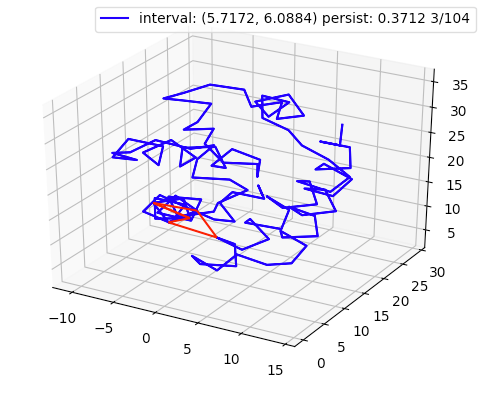
\includegraphics[width=\linewidth]{img/hom/Simplex1.png}
    \caption{Persistent Homology detecting a small cycle. This small hole doesn't seem indicative of any important feature of our protein. }
    \label{Simplex1}
\end{figure}

\begin{figure}[H]
    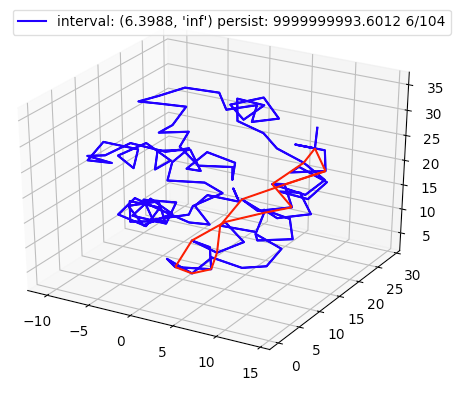
\includegraphics[width=\linewidth]{img/hom/Simplex2.png}
    \caption{Persistent homology detecting an alpha helix. The hole is a significant feature of our data since the hole persists for a long time.}
    \label{Simplex2}
\end{figure}

\begin{figure}[H]
    \includegraphics[width=\linewidth]{img/hom/Simplex3.png}
    \caption{Persistent homology detecting a beta sheet. This hole is a significant feature of our data since the hole persists for a long time.}
    \label{Simplex3}
\end{figure}

We inspect some key holes generated by the persistent homology to see if it captures the  features of our data well. We see that persistent homology is able to detect the presence of alpha helices (Fig.\ref{Simplex2}) and beta sheets (Fig.\ref{Simplex3}). The persistent homology is on par with the distance matrix because it can represent alpha helices and beta sheets. However, the information of the birth and the death of the holes alone aren't enough to describe relationships between multiple pairs of alpha helices.

\subsubsection{ Sparse Matrix}

A series of matrices were used during the computation of the persistence homology. We note that in D1, D2, R1, R2, V1, V2, B, Z, Main matrices we see that the most of the matrix consists of zero elements (Fig.\ref{1ux8MainMatrix}). An performance evaluation of the homology algorithm showed that a lot of time was spent on manipulating the matrix object which was implemented in numpy. This is because most matrices have dimensions which are well over 1000x1000.


\begin{figure*}
	\centering
    \includegraphics[width=\linewidth]{img/homex/main.png}
    \caption{Here we see the main matrix of persistent homology for our collection of 17 points. We note that most of the matrix consists of zero elements}
    \label{1ux8MainMatrix}
\end{figure*}

A sparse matrix was implemented so that we do not keep track of the zero values. For a NxM matrix, a list of length M holds dictionaries whose keys range over the row numbers less than or equal to N and whose values are the values of the nonzero elements. For a matrix given in (Fig.\ref{spmat}), the corresponding sparse matrix would be (Fig.\ref{sparseImpl}).

\begin{figure}[H]
    \includegraphics[width=\linewidth]{img/sparseM/sparseMat}
    \caption{Here is small matrix where most of the matrix consists of zeroes. We will implement this into a sparse matrix to improve the computation time of the persistence algorithm.}
    \label{spmat}
\end{figure}

\begin{figure}[H]
    \includegraphics[width=\linewidth]{img/sparseM/sparseMat}
    \caption{Here is the implementation of the matrix with zeroes as a sparse matrix. Although the computational benefits of using the sparse matrix over a regular matrix isn't huge for small matrices, the matrices used in persistent homology much larger than 1000x1000}
    \label{sparseImpl}
\end{figure}

When we add a new value at the (i,j) coordiantes of the sparse matrix, we update our matrix using the jth column dictionary and the i key. Whenever an operation is performed that can change the ij th value of a matrix to zero, i key is removed from the jth column dictionary.

Implementing these changes to the matrix made the computation speed of the persistent homology for SCOP 1.55 10 times faster.

\subsubsection{ Backbone Aware Persistence Homology}

The computation of persistent homologies for $\dfrac{1}{10}$ of SCOP 1.55, took around 15 hours. Upon inspect of the computation times, we noted that proteins that took longer than 50 seconds to compute the persistence homology accounted for about 11 hours of the 15 hours. 

The reason why persistent homology had a difficult time was due to a improperly set cutoff value. Initially we set the cutoff value as the maximum length of the edges found in the protein backbone. This was because we wanted to include the edges of the protein backbone as part of the filtration of $\epsilon$ Vietoris-Rips simplicial complexes because it is a very important feature of the protein. However, some of the proteins had very long edges in the protein backbone chain, making the cutoff value very large and making our algorithm compute the persistent homology for all the edges in our protein. When we adjusted the cutoff value to be just around 6 Å we noticed that beta helices along the protein were not being captured very well by the holes.

To remedy this issue, we multiply a weight of $.25$ on the edges belonging to the protein backbone. This would ensure that protein backbone edges that reasonably small would get included as part of the filtration of $\epsilon$ Vietoris-Rips simplicial complexes. Placing this modification greatly sped up the speed of the computation of persistent homologies, computing $\dfrac{1}{10}$ of SCOP 1.55 from 15 hours to 2.6 seconds.

\subsubsection{ Persistence Images}

\begin{figure}
    \includegraphics[width=\linewidth]{persistenceimages.png}
    \caption{For a protein, a plot of the barcodes is constructed on a 2D plane where x-coordinate is the birth and the y-coordinate is the persistence. Then, a blurred resolution of the plot is taken as the persistent image.}
    \label{persistenceimages}
\end{figure}

The persistent homology of each protein is converted into an input feature called persistent images (Fig.\ref{persistenceimages}). For each bar in the barcode, we plot it on a 2-dimensional vector space with the x coordinate being the birth and the y coordinate being the persistence of the hole. For the simplices that persist infinitely, we plot the y coordinates well above the maximum value for persistence. After the plot is constructed, a 2D histogram is created of the data. The resolution of the histogram is 100x100 and the x interval and the y interval have been selected by looking at the x and y values of the plots for all proteins (Fig.\ref{xhist}) \& Fig.\ref{yhist})

\begin{figure}
    \includegraphics[width=\linewidth]{xhist.png}
    \caption{We inspect the x values, birth values, of barcodes of all the proteins prior to selecting an x interval for the 2D histogram.}
    \label{xhist}
\end{figure}
\begin{figure}
    \includegraphics[width=\linewidth]{yhist.png}
    \caption{We inspect the y values, persistent values, of the barcodes of all the proteins prior to selecting an y interval for the 2D histogram.}
    \label{yhist}
\end{figure}

This representation captures the essential information about each simplex as well as ordering them. The more persistent simplices are higher and the simplices that are born later appear towards the right.  Fig.\ref{bcodeImg} shows this plot for the protein 1ux8.

\begin{figure}
    \includegraphics[width=\linewidth]{img/barcode2}
    \caption{Here is the plot of the persistence homology for the protein 1ux8. The x axis is the birth of the hole and the y axis is the persistence of the hole. At the very top we plot the simplices with infinite persistence.}
    \label{bcodeImg}
\end{figure}
----------------------
\subsection{Convolutional Network Model}
%----------------------

The features from each of these subsections were fed into a a 2D-convolutional network. The architecture of the 2D-convolutional network for mapping protein structure to folds contains, in order, 32 3x3 convolutional layers, 64 3x3 convolutional layers, 2x2 max pooling, 128 dense layer, and the output layer.

\begin{figure}
\includegraphics[width=.9\linewidth]{model_plot.png}
\caption{The architecture of a 2D deep convolutional network for protein fold classification. Convolutional layers were added as part of a traditional image classification network. Dense layers were added to help the network use the discovered features in the images. A dropout layer was added to make our network learn an ensemble of different models}
\label{model_plot}
\end{figure}

This is a relatively simple network. However, for our task of classifying quarter million of proteins, it performs exceptionally well. There are a lot of benefits for a simple network performing well. First, it ensures that the model is not overfitting the data. Second, it allows for the network to train at a reasonable speed.

We outline the hyper-parameters that were used for traing our convolutional neural network. For all of the training, a batch size of 50 was used. Stochastic gradient descent with a learning rate of $.01$ was used. The labels of the protein folds were one hot encoded as a vector of size 605 for SCOP 1.55 and 1232 for SCOPe 2.07. For SCOP 1.55 the models were trained for 20 epochs. SCOPe 2.07, the models were trained for 30 epochs.


% ===============================================================
\section{Results}
% ===============================================================

Overall, the distance matrix out performs persistent homology as an input feature on both SCOP 1.55 and SCOPe 2.07. On SCOP 1.55 the distance matrix has an accuracy of 86\% and the persistence homology has an accuracy of 62\%. On SCOPe 2.07, the distance matrix has an accuracy of 90\% and the persistence homology has an accuracy of 54\%. 

The distance matrix performs a lot better than the persistence homology because the distance matrix conveys spatial relationship between the alpha helices and beta sheets while the persistence images do not. The specifically, persistence homology would have trouble distinguishing between proteins of Alpha/Beta and Alpha+Beta classes since these proteins are both composed of alpha helices and beta sheets but their spatial orientations are different. 

We note that the distance matrix performs better on SCOPe 2.07 than SCOP 1.55. This is likely due to the increase in the amount of training data per fold. The number of classification labels increased 2 fold but the amount of data increased 8 fold between SCOP 1.55 and SCOPe 2.07. 

Finally, the persistence homology performs worse in SCOPe 2.07 than SCOP 1.55. Although there are more training data per fold in SCOPe 2.07, there are more proteins that which require more information about the spatial orientation of beta sheets and alpha helices were added in SCOPe 2.07. This makes it more difficult for persistence homology to be accurate.

We found that the sparse distance matrix and the regular distance matrix perform similarly. The sparse distance matrix does take more epochs for it to reach the similar level of accuracy as the regular distance matrix.

\begin{table}[H]
    \centering
    \begin{tabular}{| l | l | l |}
        \hline 
        Method & SCOP 1.55 & SCOPe 2.07  \\ \hline
        \textbf{\makecell{Distance\\ Matrix}} & 86\% & 90\%  \\ \hline
        \textbf{\makecell{Persistence\\ Homology}} & 62\% & 54\%  \\ \hline
    \end{tabular}
    \caption{ }
    \label{}
\end{table}




%------------------------------------------------
%
%\section{Table, Figure, List Examples}
%
%\begin{figure}
%  \includegraphics[width=\linewidth]{xhist.png}
%  \caption{A boat.}
%  \label{fig:boat1}
%\end{figure}
%
%\begin{table}[]
%\begin{tabular}{ccc}
%\hline
% a & a & a \\ \hline
% a & a & a \\
% a & a & a \\
% a & a & a
%\end{tabular}
%\end{table}
%
%
%\begin{itemize}
%   \item First item in a list 
%   \item Second item in a list 
%   \item Third item in a list
%\end{itemize}
%
%\begin{description}
%   \item[First] This is the first item
%   \item[Last] This is the last item
%\end{description}
%
%\begin{enumerate}
%   \item First numbered item in a list
%   \item Second numbered item in a list
%   \item Third numbered item in a list
%\end{enumerate}


%-------------------------------
%   BIBLIOGRAPHY
%---------------------------------
\pagebreak
\pagebreak
\begin{thebibliography}{9}
%APA Style
\bibitem{persistenceImages} 
Henry Adams, Tegan Emerson, and Michael Kirby. 
2017.
\textit{Persistence Images: A Stable Vector Representation of
Persistent Homology}. 
Journal of Machine Learning Research 18 (2017) 1-35

\bibitem{deepsf}
Jie Hou, Badri Adhikari and Jianlin Cheng.
2018.
\textit{DeepSF: deep convolutional neural network for mapping protein sequences to folds}
Bioinformatics, 34(8), 2018, 1295–1303

\bibitem{sakai}
Katsuro Sakai.
2010.
\textit{Simplicial Homology — A Short Course}
Institute of Mathematics University of Tsukuba

\bibitem{scope}
Fox NK, Brenner SE, Chandonia JM.
2014.
\textit{SCOPe: Structural Classification of Proteins—extended, integrating SCOP and ASTRAL data and classification of new structures.}
Nucleic Acids Research 42:D304-309. doi: 10.1093/nar/gkt1240

\bibitem{SCOP}
Murzin AG, Brenner SE, Hubbard TJP, Chothia C. 1995. SCOP: a structural classification of proteins database for the investigation of sequences and structures. Journal of Molecular Biology 247:536-540.

\bibitem{fastSCOP}
Fast SCOP Classification of Structural Class and Fold Using Secondary
Structure Mining in Distance Matrix
Jian-Yu Shi and Yan-Ning Zhang

\bibitem{pdb}
Protein Data Bank Guide
\textit{Protein Data Bank Changes Guide
    New Changes in Version 3.20}
Nucleic Acids Research 42:D304-309. doi: 10.1093/nar/gkt1240
https://cdn.rcsb.org/wwpdb/docs/documentation/file-format/changesv3.20.pdf

\bibitem{SCOPHom}
Cang Z, Mu L, Wu K, Opron K, Xia K, Wei GW. A topological approach for protein classification. Molecular based Mathematical Biology. 2015;3:140–162.

%figures

\bibitem{fig:convexHull}
[Untitled illustration of convex hull]. Retrieved April 23, 2019
             from http://mathworld.wolfram.com/ConvexHull.html
             
\bibitem{fig:n-simplices}
[Untitled illustration of simplices]. Retrieved April 23, 2019
https://www.researchgate.net/figure/Simplices-from-0-simplex-to-3-simplex-11\_fig7\_290190525

\bibitem{fig:rips-complex}
[Untitled illustration of Vietoris-Rips-complex]. Retrieved April 23, 2019
https://www.researchgate.net/figure/Computation-of-PH-for-a-point-cloud-using-the-Vietoris-Rips-complex\_fig1\_279633447

\bibitem{fig:simpcomplex}
[A simplicial 3-complex]. Retrieved April 23, 2019 https://www.wikiwand.com/en/Simplicial\_complex

\bibitem{fig:simpcomplex}
https://www.researchgate.net/figure/Persistent-homology-of-a-sample-of-genetic-sequences-Barcode-and-simplicial-complexes\_fig4\_277022824
\end{thebibliography}

\end{document}
